\documentclass{article}[a4paper,12pt]
\usepackage[utf8]{inputenc}
\usepackage{amsmath,amssymb,amsthm,amsfonts,mathtools}
\usepackage[inline]{enumitem}
\usepackage{soul}
\usepackage{cancel}
\usepackage{hyperref}
\usepackage{centernot}
\usepackage{pifont}
\usepackage{changepage}
\usepackage{subcaption}
\usepackage[section]{placeins}
\usepackage{lipsum, graphicx, caption}
\usepackage{float}
\usepackage{commath}

\theoremstyle{definition}
\newtheorem{innercustomgeneric}{\customgenericname}
\providecommand{\customgenericname}{}
\newcommand{\newcustomtheorem}[2]{%
  \newenvironment{#1}[1]
  {%
   \renewcommand\customgenericname{#2}%
   \renewcommand\theinnercustomgeneric{##1}%
   \innercustomgeneric
  }
  {\endinnercustomgeneric}
}
\newcustomtheorem{customthm}{Theorem}
\newcustomtheorem{customlem}{Lemma}
\newcustomtheorem{customdefn}{Definition}
\newcustomtheorem{customprop}{Proposition}
\newcustomtheorem{customexer}{Exercise}
\renewcommand{\qedsymbol}{$\blacksquare$}

\setlength\parindent{0pt}
\let\emptyset\varnothing
\usepackage{geometry}
\geometry{
	a4paper, portrait,
	total = {170mm,257mm},
	left = 20mm,
	top = 20mm,
}

\usepackage{xcolor}
\usepackage{pagecolor}
\pagecolor{white}
\color{black}

\title{\textbf{Introduction to Game Developement}}
\author{
	\textbf{Om Prabhu}\\
	19D170018\\
	Undergraduate, Department of Energy Science and Engineering\\
	Indian Institute of Technology Bombay\\}
\date{Last updated \today}

\begin{document}
\maketitle
\vspace{-12pt}
\hrulefill
\vspace{6pt}

\textbf{NOTE:} This document is a short compilation of my notes taken during a course in game design and development. You are free to use it and my project files for your own personal use \& modification. You may check out the course here: \texttt{\href{https://www.coursera.org/learn/game-development?specialization=game-development}{https://www.coursera.org/learn/game-development?specialization=game-development}}.

\hrulefill
\tableofcontents
\pagebreak

\section{Introduction}
\subsection{About myself}
Hello. I am Om Prabhu, currently an undergrad at the Department of Energy Science and Engineering, IIT Bombay. If you have gone through my website (\texttt{\href{https://omprabhu31.github.io}{https://omprabhu31.github.io}}) earlier, which is probably where you found this document too, you will know that I love playing video games, story-rich titles in particular. I also listen to a lot of music and engage in a little bit of creative writing as and when I get time. With this brief self-introduction, let's get into what actually motivated me to pursue game development.

\subsection{Motivation}
Most of my motivation for pursuing game development came from playing games itself. I am talking less of titles like \textit{Grand Theft Auto}, generic FPS/RPGs, etc meant purely for self-entertainment and more about games like \textit{Life is Strange}, \textit{When the Darkness Comes}, etc that actually give you some amazing stories and/or simple, powerful messages to be remembered for life. When one has experiences like this, the question naturally hangs at the back of their minds - why not create enriching experiences like this?
\vspace{6pt}

Now while playing games (of all genres) is vital to understanding what essentially makes a good game, they are two very different things - it's like comparing movie binging to actually making movies. Making games involves a lot of hardwork at different stages of the development process and there is a reason why good game developers take their time (often more than 10 years) before putting out a game on the market.
\vspace{12pt}

Nevertheless, I decided to give it a shot - the worst that could happen is I could end up hating it, but I hate it during quarantine anyway.

\hrulefill
\vspace{6pt}

\textbf{NOTE:} 
\begin{enumerate}
	\item This entire course works with Unity3D as the game engine, however the exact same concepts apply to other engines like Unreal, Godot, etc as well.
	\item The source files for course projects are available on my website for free use and modification. I will mainly be working with the 2019.4.2f1 and 2017.4.40f1 LTS releases of Unity, so you might need to install these versions of the engine before you try them out.
	\item Most of the project builds will be for the WebGL platform. Many browsers do not support running local WebGL content out of the box. You might find this guide handy: \texttt{\href{techwiser.com/enable-webgl}{techwiser.com/enable-webgl}}
\end{enumerate}
\hrulefill
\pagebreak

\section{Overview of Game Development}
\subsection{Factors to consider before starting out}
\begin{center}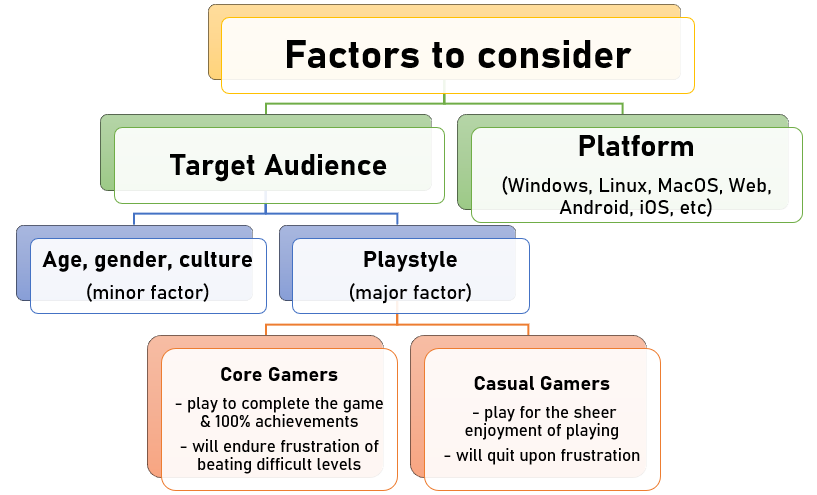
\includegraphics[scale=0.8]{gamedev_basic_factors_to_consider.png}\end{center}

\subsection{Hierarchy of game structure}
Keeping in mind the above factors, we proceed to conceptualize the game structure.
\begin{center}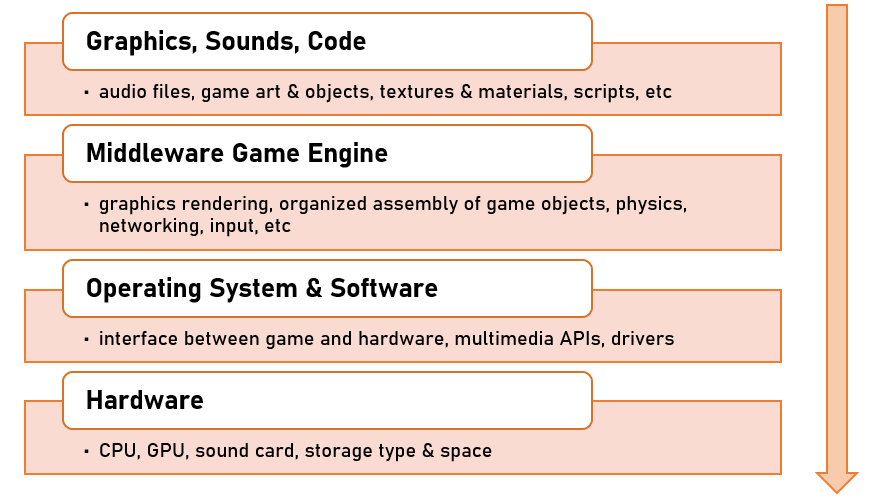
\includegraphics[scale=0.8]{game_design_hierarchy.png}\end{center}

While normally we would construct anything from the ground up, from a game design perspective things work better when conceptualized from the top down. 
\begin{itemize}
	\item We first create everything essential, i.e. `game assets' - that would mean any art, textures \& materials, game object models, audio/music and scripts (basically code that defines interaction between objects)
	\item Then, we actually construct the levels in the game using the above created assets in an engine like Unity, Unreal, Godot, etc
	\item We then build the game for the intended platforms
	\item Finally the game is tested for bugs and to determine the requirements for a system that could hope to run our game
\end{itemize}

\subsection{Team structure and roles}
Considering all the stuff from the previous subsection, it would be near impossible for a single person to carry out all the work required and make an end product that ticks all the boxes (individual developers do exist still). This is why there are often teams, ranging in size from as small as 2-3 people to well over 1000 employees, with each member having one or more roles to perform.
\begin{itemize}
	\item Game Designer: execution of the idea behind the story, designing levels, gameplay mechanics, organizing assets and documents
	\item Story Designer: character design, story arcs, writing dialogues, etc
	\item Game Producer: monitoring project budgets, keeping track of deadlines, keeping the team together
 	\item Programmer: writing actual code to determine how game objects interact
	\item Game Artist: create concept art, textures for game objects to give them unique looks 
	\item Sound Designer: create and edit music to match the mood of various in-game scenes
	\item Game Tester: not the same as a player; requires sitting on a single game level for hours to identify bugs/inconsistencies
\end{itemize}
\hrulefill

\end{document}
